% Options for packages loaded elsewhere
\PassOptionsToPackage{unicode}{hyperref}
\PassOptionsToPackage{hyphens}{url}
\PassOptionsToPackage{dvipsnames,svgnames,x11names}{xcolor}
%
\documentclass[
  letterpaper,
  DIV=11,
  numbers=noendperiod]{scrartcl}

\usepackage{amsmath,amssymb}
\usepackage{lmodern}
\usepackage{iftex}
\ifPDFTeX
  \usepackage[T1]{fontenc}
  \usepackage[utf8]{inputenc}
  \usepackage{textcomp} % provide euro and other symbols
\else % if luatex or xetex
  \usepackage{unicode-math}
  \defaultfontfeatures{Scale=MatchLowercase}
  \defaultfontfeatures[\rmfamily]{Ligatures=TeX,Scale=1}
\fi
% Use upquote if available, for straight quotes in verbatim environments
\IfFileExists{upquote.sty}{\usepackage{upquote}}{}
\IfFileExists{microtype.sty}{% use microtype if available
  \usepackage[]{microtype}
  \UseMicrotypeSet[protrusion]{basicmath} % disable protrusion for tt fonts
}{}
\makeatletter
\@ifundefined{KOMAClassName}{% if non-KOMA class
  \IfFileExists{parskip.sty}{%
    \usepackage{parskip}
  }{% else
    \setlength{\parindent}{0pt}
    \setlength{\parskip}{6pt plus 2pt minus 1pt}}
}{% if KOMA class
  \KOMAoptions{parskip=half}}
\makeatother
\usepackage{xcolor}
\setlength{\emergencystretch}{3em} % prevent overfull lines
\setcounter{secnumdepth}{-\maxdimen} % remove section numbering
% Make \paragraph and \subparagraph free-standing
\ifx\paragraph\undefined\else
  \let\oldparagraph\paragraph
  \renewcommand{\paragraph}[1]{\oldparagraph{#1}\mbox{}}
\fi
\ifx\subparagraph\undefined\else
  \let\oldsubparagraph\subparagraph
  \renewcommand{\subparagraph}[1]{\oldsubparagraph{#1}\mbox{}}
\fi


\providecommand{\tightlist}{%
  \setlength{\itemsep}{0pt}\setlength{\parskip}{0pt}}\usepackage{longtable,booktabs,array}
\usepackage{calc} % for calculating minipage widths
% Correct order of tables after \paragraph or \subparagraph
\usepackage{etoolbox}
\makeatletter
\patchcmd\longtable{\par}{\if@noskipsec\mbox{}\fi\par}{}{}
\makeatother
% Allow footnotes in longtable head/foot
\IfFileExists{footnotehyper.sty}{\usepackage{footnotehyper}}{\usepackage{footnote}}
\makesavenoteenv{longtable}
\usepackage{graphicx}
\makeatletter
\def\maxwidth{\ifdim\Gin@nat@width>\linewidth\linewidth\else\Gin@nat@width\fi}
\def\maxheight{\ifdim\Gin@nat@height>\textheight\textheight\else\Gin@nat@height\fi}
\makeatother
% Scale images if necessary, so that they will not overflow the page
% margins by default, and it is still possible to overwrite the defaults
% using explicit options in \includegraphics[width, height, ...]{}
\setkeys{Gin}{width=\maxwidth,height=\maxheight,keepaspectratio}
% Set default figure placement to htbp
\makeatletter
\def\fps@figure{htbp}
\makeatother

\KOMAoption{captions}{tableheading}
\makeatletter
\@ifpackageloaded{tcolorbox}{}{\usepackage[many]{tcolorbox}}
\@ifpackageloaded{fontawesome5}{}{\usepackage{fontawesome5}}
\definecolor{quarto-callout-color}{HTML}{909090}
\definecolor{quarto-callout-note-color}{HTML}{0758E5}
\definecolor{quarto-callout-important-color}{HTML}{CC1914}
\definecolor{quarto-callout-warning-color}{HTML}{EB9113}
\definecolor{quarto-callout-tip-color}{HTML}{00A047}
\definecolor{quarto-callout-caution-color}{HTML}{FC5300}
\definecolor{quarto-callout-color-frame}{HTML}{acacac}
\definecolor{quarto-callout-note-color-frame}{HTML}{4582ec}
\definecolor{quarto-callout-important-color-frame}{HTML}{d9534f}
\definecolor{quarto-callout-warning-color-frame}{HTML}{f0ad4e}
\definecolor{quarto-callout-tip-color-frame}{HTML}{02b875}
\definecolor{quarto-callout-caution-color-frame}{HTML}{fd7e14}
\makeatother
\makeatletter
\makeatother
\makeatletter
\makeatother
\makeatletter
\@ifpackageloaded{caption}{}{\usepackage{caption}}
\AtBeginDocument{%
\ifdefined\contentsname
  \renewcommand*\contentsname{Table of contents}
\else
  \newcommand\contentsname{Table of contents}
\fi
\ifdefined\listfigurename
  \renewcommand*\listfigurename{List of Figures}
\else
  \newcommand\listfigurename{List of Figures}
\fi
\ifdefined\listtablename
  \renewcommand*\listtablename{List of Tables}
\else
  \newcommand\listtablename{List of Tables}
\fi
\ifdefined\figurename
  \renewcommand*\figurename{Figure}
\else
  \newcommand\figurename{Figure}
\fi
\ifdefined\tablename
  \renewcommand*\tablename{Table}
\else
  \newcommand\tablename{Table}
\fi
}
\@ifpackageloaded{float}{}{\usepackage{float}}
\floatstyle{ruled}
\@ifundefined{c@chapter}{\newfloat{codelisting}{h}{lop}}{\newfloat{codelisting}{h}{lop}[chapter]}
\floatname{codelisting}{Listing}
\newcommand*\listoflistings{\listof{codelisting}{List of Listings}}
\usepackage{amsthm}
\theoremstyle{plain}
\newtheorem{theorem}{Theorem}[section]
\theoremstyle{definition}
\newtheorem{definition}{Definition}[section]
\theoremstyle{remark}
\renewcommand*{\proofname}{Proof}
\newtheorem*{remark}{Remark}
\newtheorem*{solution}{Solution}
\makeatother
\makeatletter
\@ifpackageloaded{caption}{}{\usepackage{caption}}
\@ifpackageloaded{subcaption}{}{\usepackage{subcaption}}
\makeatother
\makeatletter
\@ifpackageloaded{tcolorbox}{}{\usepackage[many]{tcolorbox}}
\makeatother
\makeatletter
\@ifundefined{shadecolor}{\definecolor{shadecolor}{rgb}{.97, .97, .97}}
\makeatother
\makeatletter
\makeatother
\ifLuaTeX
  \usepackage{selnolig}  % disable illegal ligatures
\fi
\IfFileExists{bookmark.sty}{\usepackage{bookmark}}{\usepackage{hyperref}}
\IfFileExists{xurl.sty}{\usepackage{xurl}}{} % add URL line breaks if available
\urlstyle{same} % disable monospaced font for URLs
\hypersetup{
  colorlinks=true,
  linkcolor={blue},
  filecolor={Maroon},
  citecolor={Blue},
  urlcolor={Blue},
  pdfcreator={LaTeX via pandoc}}

\author{}
\date{}

\begin{document}
\ifdefined\Shaded\renewenvironment{Shaded}{\begin{tcolorbox}[interior hidden, frame hidden, boxrule=0pt, breakable, borderline west={3pt}{0pt}{shadecolor}, enhanced, sharp corners]}{\end{tcolorbox}}\fi

\hypertarget{section-2}{%
\section*{Section 2}\label{section-2}}
\addcontentsline{toc}{section}{Section 2}

Last Updated: 21 Sept 2023

Date: 22 Sept 2023

\hypertarget{introduction}{%
\subsection{Introduction}\label{introduction}}

In this section, we will discuss:

\begin{itemize}
\tightlist
\item
  Reasoning by Representation
\item
  Derivation path of distribution representations
\item
  Poisson Processes
\end{itemize}

\hypertarget{reasoning-by-representation}{%
\subsection{Reasoning by
Representation}\label{reasoning-by-representation}}

Some of the important terms and definitons of Chapter 3 is as follow:

\begin{enumerate}
\def\labelenumi{\arabic{enumi}.}
\item
  \textbf{Bernoulli}: A random variable \(Y\) has the \emph{Bernoulli
  distribution} with parameter \(p\), denoted \(Y\sim Bern(p)\), if
  \(P(Y=1)=p\) and \(P(Y=0)=1-p\)
\item
  \textbf{Binomial}: sum of \(n\) iid Bernoulli random variables
\item
  \textbf{Uniform}: \(U = \sum_{i=1}^\infty \frac{B_i}{2^i} \sim\) Unif
  where \(B_i\) iid \(Bern(0.5)\).
\item
  \textbf{PIT sampling}: Let \(F\) be \textit{any} CDF with quantile
  function \(F^{-1}\), let \(U \sim Unif\) then \(F^{-1}(U) \sim F.\)
\item
  \textbf{PIT pivoting}: Let \(F\) be a continuous CDF, and
  \(Y \sim F\), then \(F(Y)\sim Unif.\)
\item
  \textbf{Exponential}: Let \(U\sim\) Unif. Then
  \(X = -\log U \sim \textnormal{Expo}.\)
\item
  \textbf{Gamma}: For a positive integer \(n\),
  \(G_n= X_1+X_2+\cdots + X_n \sim Gamma(n)\), where
  \(X_i \overset{i.i.d}{\sim}\) Expo.
\item
  \textbf{Laplace} : \(L \sim \textnormal{Laplace}\) if \(L \sim SX\)
  where \(S\) is random sign and \(X\sim Expo.\)
\item
  \textbf{Weibull}: \(W = X^\beta \sim\) Wei(\(\beta\)) where
  \(X \sim Expo\) and \(\beta >0.\)
\item
  \textbf{Beta}: \(B = \frac{G_a}{G_a+G_b} \sim Beta(a,b)\) where \$
  G\_a\sim Gamma(a)\$, \(G_b\sim Gamma(b)\) and
  \(G_a \perp\!\!\!\!\perp G_b\); note that
  \(U^{1/\alpha} \sim Beta(\alpha,1).\)
\item
  \textbf{Beta-Gamma}: Let
  \(G_a \sim Gamma(a) \perp\!\!\!\!\perp G_b\sim Gamma(b)\) ,
  \(B = \frac{G_a}{G_a+G_b}\) and \(T = G_a + G_b \sim Gamma(a+b).\)
  Then \(T \perp\!\!\!\!\perp B.\)
\item
  \textbf{Chi-squared}: \(G \sim \chi_n^2\) if
  \(G\sim 2Gamma\left(\frac{n}{2}\right).\)
\item
  \textbf{Normal}: \(Z = SX \sim \mathcal{N}(0,1)\) where \(S\) is
  random sign and \(X\sim \chi_1.\)
\item
  \textbf{Box-Muller}: \(U_1,U_2 \overset{i.i.d}{\sim}\)Unif. Then
  \(\sqrt{-2\ln U_2}\cos{(2\pi U_1)}, \sqrt{-2\ln U_2}\sin{(2\pi U_1)} \overset{i.i.d}{\sim} \mathcal{N}(0,1)\)
\item
  \textbf{Student \(t\)-distribution}:
  \(T = \frac{Z}{\sqrt{V_n/n}} \sim t_n\) where
  \(Z \sim N(0,1) \perp\!\!\!\!\perp V_n \sim \chi_n^2.\)
\item
  \textbf{Cauchy}:
  \(C = \frac{Z_1}{Z_2} \sim \textnormal{Cauchy} \sim t_1\) where
  \(Z_1,Z_2 \sim_{i.i.d} \mathcal{N}(0,1)\).
\end{enumerate}

For ease of referencing, Eric Zhang have summarized how to move from one
distribution to next in a figure, in which we will discuss in the next
section.

\hypertarget{derivation-path-of-distribution-representations}{%
\subsection{Derivation path of distribution
representations:}\label{derivation-path-of-distribution-representations}}

Below is a pitcure showing derivation path of distribution
representations, kindly created by
\href{https://www.ekzhang.com/assets/pdf/Stat_210_Notes.pdf}{Eric
Zhang}:

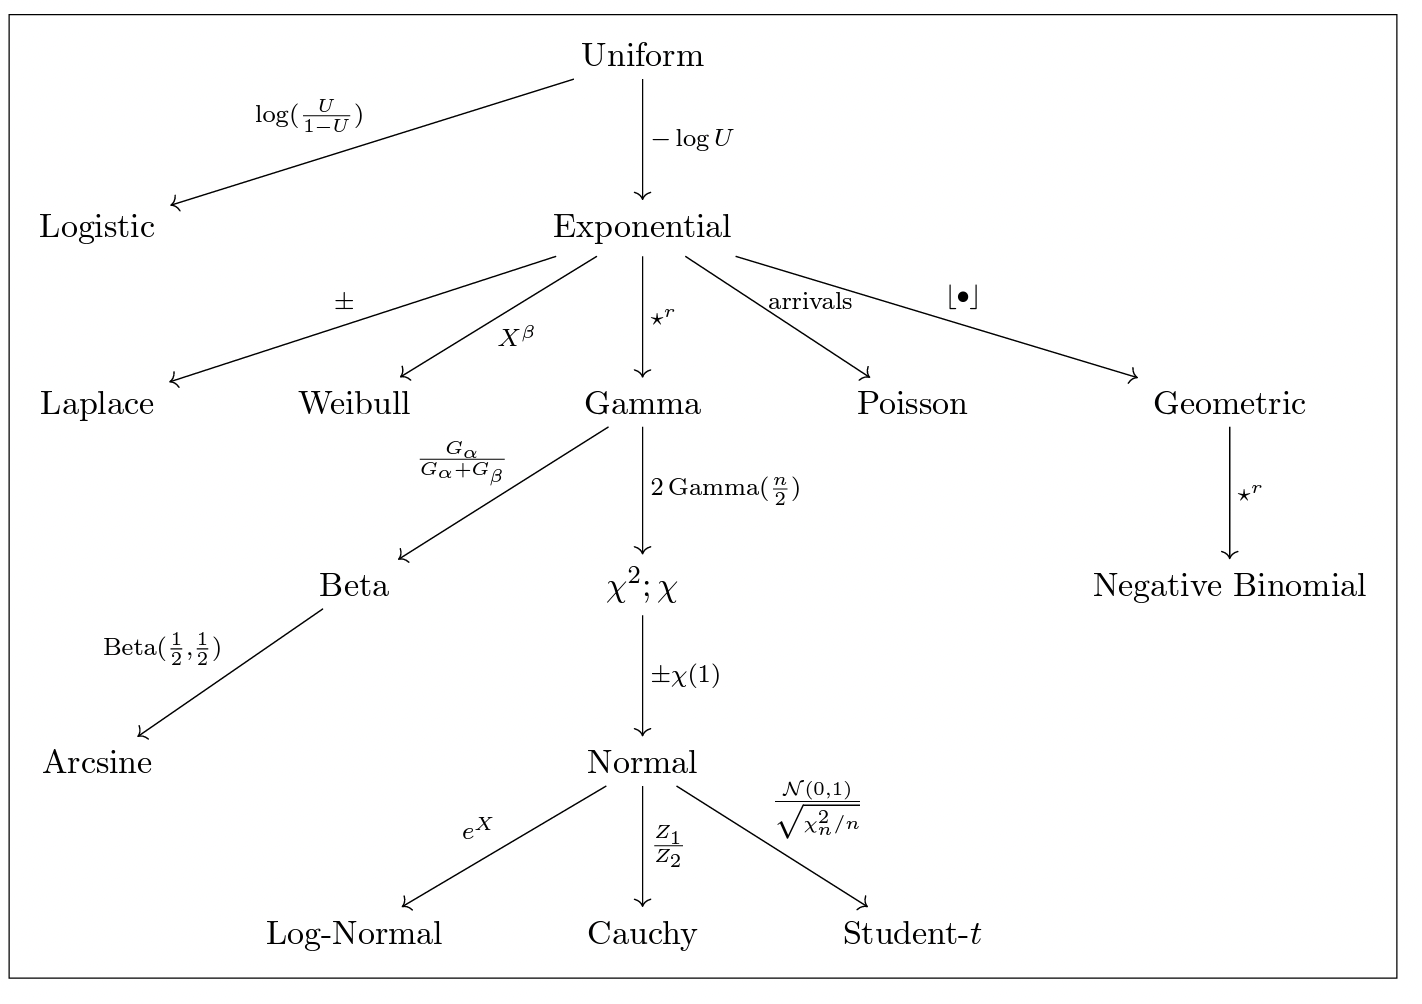
\includegraphics{assets/img/derivation.png}

\hypertarget{pencil-3.3.2}{%
\subsubsection{✏️ Pencil 3.3.2}\label{pencil-3.3.2}}

Show that if \(U\sim Unif\), then \(1-U \sim Unif\). Also, show that
\(2U-1 \sim SU\) for \(S\) a random sign independent of \(U\) (so
\(2U-1\) is symmetric about 0, while \(U\) is symmetric about \(1/2\);
see Section 3.10 for more information.)

\begin{tcolorbox}[enhanced jigsaw, leftrule=.75mm, rightrule=.15mm, breakable, colback=white, toprule=.15mm, opacityback=0, arc=.35mm, colframe=quarto-callout-tip-color-frame, left=2mm, bottomrule=.15mm]
\begin{minipage}[t]{5.5mm}
\textcolor{quarto-callout-tip-color}{\faLightbulb}
\end{minipage}%
\begin{minipage}[t]{\textwidth - 5.5mm}

\textbf{Solution}\vspace{2mm}

If \(U\sim Unif\), \(1-U=1+(0-1)U\) is Uniform between 1 and 0 so
\(1-U \sim Unif\) as well.

\(2U-1 = -1 +(1-(-1))U\) is Uniform between \(-1\) and 1, and SU is also
Uniform between -1 and 1 by definition, so \(2U-1 \sim SU\)

\end{minipage}%
\end{tcolorbox}

\hypertarget{pencil-3.4.12}{%
\subsubsection{✏️ Pencil 3.4.12}\label{pencil-3.4.12}}

Let \(Y_1\) and \(Y_2\) be r.v.s (possibly deifnied on different
\(\Omega\)'s) with CDFs \(F_1\) and \(F_2\) respectively. A commonly
used partial order on distributions (and thus on r.v.s),
\emph{stochastic domination} is defined by the relation
\(Y_1 \preceq Y_2\) iff \(F_1(y) \geq F_2(y)\) for all
\(y \in \mathbb{R}\).

Find an example of \(Y_1\) and \(Y_2\) on the same space with
\(Y_1 \preceq Y_2\) but \(P(Y_1 > Y_2) \geq 0.95\)

\begin{tcolorbox}[enhanced jigsaw, leftrule=.75mm, rightrule=.15mm, breakable, colback=white, toprule=.15mm, opacityback=0, arc=.35mm, colframe=quarto-callout-tip-color-frame, left=2mm, bottomrule=.15mm]
\begin{minipage}[t]{5.5mm}
\textcolor{quarto-callout-tip-color}{\faLightbulb}
\end{minipage}%
\begin{minipage}[t]{\textwidth - 5.5mm}

\textbf{Solution}\vspace{2mm}

As in the previous clock example, we can let \(Y_1\) and \(Y_2\) be
discrete Uniform on a clock with \(\lfloor 1/0.95 \rfloor\) numbers, so
that \(Y_1 \sim Y_2\) when \(Y_1 \preceq Y_2\) . Then,
\(P(Y_1 > Y_2) \geq P(Y_1 = Y_2+1) \geq 0.95\)

\end{minipage}%
\end{tcolorbox}

\hypertarget{pencil-3.5.10}{%
\subsubsection{✏️ Pencil 3.5.10}\label{pencil-3.5.10}}

Let \(W_1 \sim Wei(\beta_1), W_2 \sim Wei(\beta_2)\). Show that
\((W_1|W_1 \geq 1) \preceq (W_2|W_2 \geq 1)\) iff
\(\beta_1 \leq \beta_2\).

\begin{tcolorbox}[enhanced jigsaw, leftrule=.75mm, rightrule=.15mm, breakable, colback=white, toprule=.15mm, opacityback=0, arc=.35mm, colframe=quarto-callout-tip-color-frame, left=2mm, bottomrule=.15mm]
\begin{minipage}[t]{5.5mm}
\textcolor{quarto-callout-tip-color}{\faLightbulb}
\end{minipage}%
\begin{minipage}[t]{\textwidth - 5.5mm}

\textbf{Solution}\vspace{2mm}

\((W_1|W_1 \geq 1) \preceq (W_2|W_2 \geq 1)\) implies that
\(F_1(w) \geq F_2(w)\), which by definition implies that
\(1-exp(-w^{1/\beta_1}) \geq 1-exp(-w^{1/\beta_2})\). This further
implies that \(exp(-w^{1/\beta_2}) \geq exp(-w^{1/\beta_1})\), which
implies that \(-w^{1/\beta_2} \geq -w^{1/\beta_1}\), whcih is similar to
\(w^{1/\beta_1} \geq w^{1/\beta_2}\), which further implies than when
\(w\geq 1\), \(\frac{1}{\beta_1} \geq \frac{1}{\beta_2}\), thus we show
that \(\beta_1 \leq \beta_2\).

\end{minipage}%
\end{tcolorbox}

\hypertarget{pencil-3.6.16}{%
\subsubsection{✏️ Pencil 3.6.16}\label{pencil-3.6.16}}

Let \(C \sim\) Cauchy and \(U \sim\) Unif. Show that
\[tan(2 \pi U) \sim C\]

\begin{tcolorbox}[enhanced jigsaw, leftrule=.75mm, rightrule=.15mm, breakable, colback=white, toprule=.15mm, opacityback=0, arc=.35mm, colframe=quarto-callout-tip-color-frame, left=2mm, bottomrule=.15mm]
\begin{minipage}[t]{5.5mm}
\textcolor{quarto-callout-tip-color}{\faLightbulb}
\end{minipage}%
\begin{minipage}[t]{\textwidth - 5.5mm}

\textbf{Solution}\vspace{2mm}

C= \(Z_1 / Z_2 = W sin (2\pi U) /W cos (2\pi U) = tan(\pi U)\)

\end{minipage}%
\end{tcolorbox}

\hypertarget{pencil-3.7.18}{%
\subsubsection{✏️ Pencil 3.7.18}\label{pencil-3.7.18}}

Show that if \(C\sim\) Cauchy, \(S\) is a random sign, and \(B\sim\)
Beta(1/2, 1/2), then
\[C+\frac{1}{C} \sim 2S\sqrt{1+C^2}\sim \frac{2S}{\sqrt{B}}\]

\begin{tcolorbox}[enhanced jigsaw, leftrule=.75mm, rightrule=.15mm, breakable, colback=white, toprule=.15mm, opacityback=0, arc=.35mm, colframe=quarto-callout-tip-color-frame, left=2mm, bottomrule=.15mm]
\begin{minipage}[t]{5.5mm}
\textcolor{quarto-callout-tip-color}{\faLightbulb}
\end{minipage}%
\begin{minipage}[t]{\textwidth - 5.5mm}

\textbf{Solution}\vspace{2mm}

\[
\begin{align*}
1+C^2 &= 1+\frac{Z_1^2}{Z_2^2} \\ 
&= \frac{Z_1^1+Z_2^2}{Z_2^2} \\
&= \frac{\chi_1}{\chi_2} \\ 
&= \frac{G_1}{G_{1/2}} \\
&= \frac{G_{1/2}+G_{1/2}}{G_{1/2}}\\
&= \frac{1}{B}
\end{align*}
\]

Thus, \(2S\sqrt{1+C^2} \sim 2S/\sqrt{B}\) follows.

Next, I am lazy to type so ask in office hour!

\end{minipage}%
\end{tcolorbox}

\hypertarget{pencil-3.9.5}{%
\subsubsection{✏️ Pencil 3.9.5}\label{pencil-3.9.5}}

Show that NBin\((r,p)\) PMF is \(P(X=x)=\) \(r+x-1 \choose x\)
\(p^r q^x\), where \(q\equiv 1-p\).

\begin{tcolorbox}[enhanced jigsaw, leftrule=.75mm, rightrule=.15mm, breakable, colback=white, toprule=.15mm, opacityback=0, arc=.35mm, colframe=quarto-callout-tip-color-frame, left=2mm, bottomrule=.15mm]
\begin{minipage}[t]{5.5mm}
\textcolor{quarto-callout-tip-color}{\faLightbulb}
\end{minipage}%
\begin{minipage}[t]{\textwidth - 5.5mm}

\textbf{Solution}\vspace{2mm}

Under convolution, we get that
\(P(X=x)=q^x p \times cdots \times q^x p (r)\) times, which can be
checked to be \(r+x-1 \choose x\) \(p^r q^x\)

\end{minipage}%
\end{tcolorbox}

\hypertarget{pencil-3.11.2}{%
\subsubsection{✏️ Pencil 3.11.2}\label{pencil-3.11.2}}

Suppose that \(Y_1, \cdots, Y_n \sim Expo\) are i.i.d. Show that the
minimum is also Exponentially distributed, with \(n\) times the rate:
\(Y_{(1)} \sim \frac{1}{n} Expo\) (the rate parameter is defined to be
reciprocal of the scale parameter)

\begin{tcolorbox}[enhanced jigsaw, leftrule=.75mm, rightrule=.15mm, breakable, colback=white, toprule=.15mm, opacityback=0, arc=.35mm, colframe=quarto-callout-tip-color-frame, left=2mm, bottomrule=.15mm]
\begin{minipage}[t]{5.5mm}
\textcolor{quarto-callout-tip-color}{\faLightbulb}
\end{minipage}%
\begin{minipage}[t]{\textwidth - 5.5mm}

\textbf{Solution}\vspace{2mm}

\[
\begin{align*}
P(min\{Y_1, \cdots, Y_n\}>y)  
&=P(Y_1 > y, \cdots, Y_n >y) \\
&=P(Y_1 > y) \cdots P(Y_n > y) \\
&= e^{-y} \cdots e^{-y} \\
&= e^{-ny} 
\end{align*}
\]

So \(P(min\{Y_1, \cdots, Y_n\}>y) = 1-e^{-ny} \sim n^{-1}Expo\)

\end{minipage}%
\end{tcolorbox}

\hypertarget{poisson-process}{%
\subsection{Poisson Process}\label{poisson-process}}

From Stat 110 textbook on pg 559:

\leavevmode\vadjust pre{\hypertarget{def-poisson-process}{}}%
\begin{definition}[]\label{def-poisson-process}

A sequence of arrivals in continuous time is a \emph{Poisson process}
with rate \(\lambda\) if the following conditions hold:

\begin{enumerate}
\def\labelenumi{\arabic{enumi}.}
\item
  The number of arrivals in an interval length \(t\) is distributed
  Pois\((\lambda t)\)
\item
  The numbers of arrivals in disjoint time intervals are independent.
\end{enumerate}

\end{definition}

Recall that in STAT 110, we also learn how to generate 1D Poisson
Process, detailed in pg 560 of the textbook:

\leavevmode\vadjust pre{\hypertarget{thm-poisson-story}{}}%
\begin{theorem}[]\label{thm-poisson-story}

(Generative Story for 1D Poisson process) To generate \(n\) arrivals
from a Poisson process on \((0, \infty)\) with rate \(\lambda\):

\begin{enumerate}
\def\labelenumi{\arabic{enumi}.}
\item
  Generate \(n\) i.i.d. Expo\((\lambda)\) r.v.s \(X_1, \cdots, X_n\)
\item
  For \(j=1, \cdots, n\), set \(T_j = X_1 + \cdots+X_j\)
\end{enumerate}

Then we can take \(T_1, \cdots, T_n\) to be the arrival times.

\emph{Ref: Story 13.1.2 in STAT 110 textbook}

\end{theorem}

Also note that on Theorem 13.2.1 in STAT 110 textbook:

\leavevmode\vadjust pre{\hypertarget{thm-conditional-counts}{}}%
\begin{theorem}[]\label{thm-conditional-counts}

(Conditional Counts) Let \((N(t):t>0)\) be a Poisson process with rate
\(\lambda\), and \(t_1<t_2\). The conditional distribution of \(N(t_1)\)
given \(N(t_2) = n\) is
\[N(t_1)|N(t_2)=n \sim Bin \left(n, \frac{t_1}{t_2}\right)\]

\end{theorem}

also note that Propositional 13.2.2 in STAT 110 textbook states that In
a Poisson process of rate \(\lambda\), conditional on \(N(t) =1\), the
first arrival time \(T_1\) has the Unif\((0,t)\) distribution.

Some other important concept about Poisson process from STAT 110
textbook include:

\leavevmode\vadjust pre{\hypertarget{thm-conditional-time}{}}%
\begin{theorem}[]\label{thm-conditional-time}

(Conditional times) In a process process of rate\(\lambda\), conditional
on \(N(t)=n\), the joint distribution of the arrival times
\(T_1, \cdots, T_n\) is the same as the joint distribution of the order
statistics of \(n\) i.i.d Unif\((0,t)\) r.v.s.

Also note that we know that the order statistics of Unif(0,1) r.v..s are
Betas, so the conditional distributions of the \(T_j\) are \emph{scaled}
Betas. To get Beta Distribution, we can just divide the \(T_j\) by \(t\)
so that their support is \((0,1)\):
\[t^{-1}T_j | N(t) = n \sim Beta(j, n-j+1)\]

\end{theorem}

\leavevmode\vadjust pre{\hypertarget{thm-poisson-story}{}}%
\begin{theorem}[]\label{thm-poisson-story}

(Generative Story for Poisson process) To generate \(n\) arrivals from a
Poisson process on \((0, t]\) with rate \(\lambda\):

\begin{enumerate}
\def\labelenumi{\arabic{enumi}.}
\item
  Generate the total number of events in the interval,
  \(N(t) \sim Pois(\lambda t)\)
\item
  Given \(N(t) = n\), generate \(n\) i.i.d Unif\((0,t)\) r.v.s
  \(U_1, \cdots, U_n\)
\item
  For \(j=1, \cdots, n\), set \(T_j = U_{(j)}\)
\end{enumerate}

\emph{Ref: Story 13.2.4 in STAT 110 textbook}

\end{theorem}

\leavevmode\vadjust pre{\hypertarget{thm-superposition}{}}%
\begin{theorem}[]\label{thm-superposition}

(Superposition). Let \((N_1(t): t>0)\) and \((N_2(t): t>0)\) be
independent Poisson process with rates \(\lambda_1\) and \(\lambda_2\)
respectively. Then the combined process \(N(t) = N_1(t) + N_2(t)\) is a
Poisson process with rate \(\lambda_1+\lambda_2\).

\end{theorem}

\leavevmode\vadjust pre{\hypertarget{thm-poisson-story-superposition}{}}%
\begin{theorem}[]\label{thm-poisson-story-superposition}

(Generative Story for superposition) To generate the superposition of
two independent Poisson processes, \((N_1(t): t>0)\) with
rate\(\lambda_1\), and \((N_2(t): t>0)\) with rate \(\lambda_2\):

\begin{enumerate}
\def\labelenumi{\arabic{enumi}.}
\item
  Generate arrivals from the Poisson process \((N_1(t): t>0)\)
\item
  Generate arrivals from the Poisson process \((N_2(t): t>0)\)
\item
  Superpose the results of steps 1 and 2.
\end{enumerate}

\emph{Ref: Story 13.2.7 in STAT 110 textbook}

\end{theorem}

There is also another generative story for superposition, as highlighted
below:

\leavevmode\vadjust pre{\hypertarget{thm-poisson-story-superposition-2}{}}%
\begin{theorem}[]\label{thm-poisson-story-superposition-2}

(Generative Story for superposition, take 2) To generate the
superposition of two independent Poisson processes, with
rate\(\lambda_1\) and \(\lambda_2\):

\begin{enumerate}
\def\labelenumi{\arabic{enumi}.}
\item
  Generate i.i.d Expo\((\lambda_1 +\lambda_2)\) r.v.s
  \(X_1, X_2,\cdots\) and let the \(j\)th arrival at time
  \(T_j =X_1+\cdots+X_j\)
\item
  Generate i.i.d r.v.s.
  \(I_1, I_2, \cdots Bern(\lambda_1/(\lambda_1+\lambda_2))\),
  independent of \(X_1, X_2, \cdots\). Let the \(j\)th arrival be type-1
  if \(I_j=1\), and type-2 otherwise.
\end{enumerate}

\emph{Ref: Story 13.2.9 in STAT 110 textbook}

\end{theorem}

Following up from the superposition definition and generative story
above, the two most important theorem arive from this are

\leavevmode\vadjust pre{\hypertarget{thm-superposition-discrete}{}}%
\begin{theorem}[]\label{thm-superposition-discrete}

(Projection of superposition into discrete time) Consider the
superposition \((N(t);t>0)\) of two independent Poisson processes with
rate \(\lambda_1\) and \(\lambda_2\). For \(j=1,2,\cdots\), let \(I_j\)
be the indicator of the \(j\)th event being from the Poisson process
with rate \(\lambda_1\). Then the \(I_j\) are i.i.d
Bern\((\lambda_1/(\lambda_1+\lambda_2))\)

\emph{Ref: Thm 13.2.11 in STAT 110 textbook}

\end{theorem}

Using the result above, we can orive wutg a story that a Gamma mixture
of Poissons is Negative Binomial:

\leavevmode\vadjust pre{\hypertarget{thm-mixture-poisson}{}}%
\begin{theorem}[]\label{thm-mixture-poisson}

(Exponential mixture of Poissons is Geometric). Suppose that
\(X \sim Expo(\lambda)\), and \(Y|X=x \sim Pois(\lambda)\). Then
\(Y\sim Geom(\lambda/(\lambda+1))\)

\emph{Ref: Thm 13.2.12 in STAT 110 textbook}

\end{theorem}

\leavevmode\vadjust pre{\hypertarget{thm-mixture-poisson-negative-binomial}{}}%
\begin{theorem}[]\label{thm-mixture-poisson-negative-binomial}

(Gamma mixture of Poissons is Negative Binomial). Suppose that
\(X \sim Gamma(r, \lambda)\), and \(Y|X=x \sim Pois(x)\). Then
\(Y\sim Nbin(r, \lambda/(\lambda+1))\)

\emph{Ref: Thm 13.2.12 in STAT 110 textbook}

\end{theorem}

\hypertarget{section-discussion-questions}{%
\subsection{Section Discussion
Questions}\label{section-discussion-questions}}

\hypertarget{section-problem-1}{%
\subsubsection{✏️ Section Problem 1}\label{section-problem-1}}

Let \(A, B, C\) be i.i.d. Uniform\((0,1)\), which are coefficients of
the following ``random'\,' quadratic equation: \[
A x^2 + 2B x + C = 0.
\] What is the probability that the above equation has real root?

\begin{tcolorbox}[enhanced jigsaw, leftrule=.75mm, rightrule=.15mm, breakable, colback=white, toprule=.15mm, opacityback=0, arc=.35mm, colframe=quarto-callout-tip-color-frame, left=2mm, bottomrule=.15mm]
\begin{minipage}[t]{5.5mm}
\textcolor{quarto-callout-tip-color}{\faLightbulb}
\end{minipage}%
\begin{minipage}[t]{\textwidth - 5.5mm}

\textbf{Solution}\vspace{2mm}

The event that the random quadratic equation has real roots is
equivalent to the event that \(4B^2 - 4AC \geq 0\) i.e.~\(B^2 \geq AC.\)
Therefore the probability that the above equation has real roots is: \[
\begin{eqnarray*}
    P(B^2 \geq AC) &=& P(2\log B \geq \log A + \log C) \\
    &=& P(-2Y_2 \geq -Y_1 - Y_3) \quad \text{where\quad$Y_1 = -  \log A, Y_2 = -  \log B, Y_3 =  - \log C$ are iid Expo's.}\\
    &=& P( 3 Y_2 \leq Y_1 + Y_2 + Y_3    )\\
    &=& P\left(  \frac{Y_2}{Y_1 + Y_2 + Y_3}  \leq \frac{1}{3}   \right) \\
    &=& P\left( \text{Beta}(1,2) \leq \frac{1}{3} \right)  \quad \text{since}\quad\frac{Y_2}{Y_1 + Y_2 + Y_3} \sim \text{Beta}(1,2)  \\
    &=& P\left(  \text{Beta}(2,1) \geq \frac{2}{3}   \right) \quad \text{since}\quad\text{Beta}(1,2) \sim 1 -  \text{Beta}(2,1) \\
    &=& P\left( U^{1/2} \geq \frac{2}{3}  \right)  \quad \text{since}\quad   \text{Beta}(2,1) \sim U^{1/2} \\
    &=& P\left( U \geq \frac{4}{9}  \right)  \\
    &=& \frac{5}{9}.
\end{eqnarray*}
\] Thus, \(2S\sqrt{1+C^2} \sim 2S/\sqrt{B}\) follows.

\end{minipage}%
\end{tcolorbox}

\hypertarget{section-problem-2}{%
\subsubsection{✏️ Section Problem 2}\label{section-problem-2}}

Assume that \(U_1, \cdots, U_n \overset{i.i.d}{\sim}\) Unif,
\(Z_1, \cdots, Z_{2n} \overset{i.i.d}{\sim} \mathcal{N}(0,1)\), and the
\(U\)'s and \(Z\)'s are independent. Define \[
X = \frac{Z_1^2 + \cdots + Z_m^2}{ Z_1^2 + \cdots + Z_{2n}^2},
\] where \(m< 2n\). Find the distribution of
\(Y = (U_1 U_2 \cdots U_n)^{-X}\).

\begin{tcolorbox}[enhanced jigsaw, leftrule=.75mm, rightrule=.15mm, breakable, colback=white, toprule=.15mm, opacityback=0, arc=.35mm, colframe=quarto-callout-tip-color-frame, left=2mm, bottomrule=.15mm]
\begin{minipage}[t]{5.5mm}
\textcolor{quarto-callout-tip-color}{\faLightbulb}
\end{minipage}%
\begin{minipage}[t]{\textwidth - 5.5mm}

\textbf{Solution}\vspace{2mm}

Let us first find the distribution of \(\log Y\). Now, \$ \log Y = - X
\log (U\_1 U\_2 \cdots U\_n) = X \sum\_\{i=1\}\^{}n ( - \log U\_i)\$.
Denoting \(G^* = \sum_{i=1}^n ( - \log U_i)\), we have
\(\log Y = XG^*\). \textbackslash{} \underline{Step-1:} We note that
\(G^*\sim \text{Gamma} (n)\) and \(X \perp\!\!\!\!\perp G^*\) (since
\(U\)'s and \(Z\)'s are independent).\textbackslash{}

Now, \(Z_i^2\sim \chi^2_1 \sim 2 \text{Gamma}(\frac{1}{2})\) for all
\(i \in \{1,2,...,2n\}\) and \(Z_i\)'s are independent. Thus, we can
represent \(X\) as \[
X\sim \frac{G_{\frac{m}{2}}}{ G_{\frac{m}{2}} + G_{n-\frac{m}{2}}} 
\] where \$ G\_\{\frac{m}{2}\} \sim \text{Gamma}(\frac{m}{2})\$,
\(G_{n-\frac{m}{2}}\sim \text{Gamma}(n-\frac{m}{2})\) and
\(G_{\frac{m}{2}} \perp\!\!\!\!\perp G_{n-\frac{m}{2}}\) . This gives us
the following.\textbackslash{} \underline{Step-2:}
\(X \sim \text{Beta}(\frac{m}{2},n-\frac{m}{2})\)

Now, we know that
\(G_{\frac{m}{2}} + G_{n-\frac{m}{2}} \sim \text{Gamma}(n)\) and
\((G_{\frac{m}{2}} + G_{n-\frac{m}{2}}) \perp\!\!\!\!\perp \frac{G_{\frac{m}{2}}}{ G_{\frac{m}{2}} + G_{n-\frac{m}{2}}}\).
This observation along with Step-1 and Step-2 implies
\[(X,G^*) \sim  \Big(\frac{G_{\frac{m}{2}}}{ G_{\frac{m}{2}} + G_{n-\frac{m}{2}}},G_{\frac{m}{2}} + G_{n-\frac{m}{2}} \Big)\]
\%Since \(G_n \sim \text{Gamma}(m/2) + \text{Gamma}(n-m/2)\) and the
representation preserves the independence between \(X\) and \(G_n\), we
have Taking the product of the components of the random vectors on both
sides, we get\textbackslash{} \underline{Step-3:}
\(\log Y \sim G_{m/2}\)\textbackslash{}

Step-3 implies, \(Y \sim e^{G_{m/2}}\). Therefore, the distribution of
\(Y\) is same as the distribution of the exponential of a
Gamma\((\frac{m}{2})\) random variable.

\end{minipage}%
\end{tcolorbox}

\hypertarget{section-problem-3}{%
\subsubsection{✏️ Section Problem 3}\label{section-problem-3}}

Let \(Z_1, Z_2 \overset{i.i.d}{\sim} \mathcal{N}(0,1)\). Furthermore,
let \(X_1,X_2 \overset{i.i.d}{\sim} \chi_1^2\). Show that \[
Z_1Z_2\sim \frac{1}{2} (X_1 - X_2).
\]

\begin{tcolorbox}[enhanced jigsaw, leftrule=.75mm, rightrule=.15mm, breakable, colback=white, toprule=.15mm, opacityback=0, arc=.35mm, colframe=quarto-callout-tip-color-frame, left=2mm, bottomrule=.15mm]
\begin{minipage}[t]{5.5mm}
\textcolor{quarto-callout-tip-color}{\faLightbulb}
\end{minipage}%
\begin{minipage}[t]{\textwidth - 5.5mm}

\textbf{Solution}\vspace{2mm}

Firstly, \((X_1,X_2) \sim (Z^2_1,Z^2_2)\). Therefore, we have \[
\frac{1}{2} (X_1 - X_2) \sim \frac{1}{2}(Z_1^2 - Z_2^2) = \frac{1}{2} (Z_1 + Z_2) (Z_1 - Z_2) .
\] Since \(Z_1 + Z_2\sim N(0, 2)\), \(Z_1 - Z_2\sim N(0, 2)\) and
\((Z_1 + Z_2)\perp\!\!\!\!\perp (Z_1 - Z_2)\) (this is one of the many
special properties of the Normal distribution), we can jointly represent
them as \((Z_1 + Z_2, Z_1-Z_2) \sim (\sqrt{2} Z_1, \sqrt{2} Z_2)\).
Consequently, we have \[
\frac{1}{2} (X_1 - X_2) \sim \frac{1}{2} \sqrt{2} Z_1 \sqrt{2} Z_2  = Z_1 Z_2.
\]

\end{minipage}%
\end{tcolorbox}

\hypertarget{section-problem-4}{%
\subsubsection{✏️ Section Problem 4}\label{section-problem-4}}

\begin{enumerate}
\def\labelenumi{(\alph{enumi})}
\item
  Let \(X_1, X_2 \overset{i.i.d}{\sim} Expo\). Show that
  \(X_1 - X_2 \sim \operatorname{Laplace}\).
\item
  Let \(Z_1,Z_2,Z_3,Z_4 \overset{i.i.d}{\sim} \mathcal{N}(0,1)\), and
  \(L \sim\) Laplace. Show that \[
  Z_1 Z_2 - Z_3 Z_4 \sim L.
  \]
\end{enumerate}

\begin{tcolorbox}[enhanced jigsaw, leftrule=.75mm, rightrule=.15mm, breakable, colback=white, toprule=.15mm, opacityback=0, arc=.35mm, colframe=quarto-callout-tip-color-frame, left=2mm, bottomrule=.15mm]
\begin{minipage}[t]{5.5mm}
\textcolor{quarto-callout-tip-color}{\faLightbulb}
\end{minipage}%
\begin{minipage}[t]{\textwidth - 5.5mm}

\textbf{Solution}\vspace{2mm}

Define \(X_1,X_2,X_3,X_4\) as \textit{i.i.d} \(\chi^2_1\) random
variables. This gives us the representation
\((X_1,X_2,X_3,X_4) \sim (Z^2_1, Z^2_2, Z^2_3, Z^2_4)\) . Now, using
problem 2.1 of this section, we have \[
Z_1 Z_2 - Z_3 Z_4 \sim \frac{1}{2} \left\{   (X_1 - X_2)  - (X_3 - X_4)    \right\} 
\sim \frac{1}{2} (Z_1^2 + Z_3^2) - \frac{1}{2} (Z_2^2 + Z_4^2).
\] By additivity of the \(\chi^2\) distribution, we have
\[\frac{Z_1^2 + Z_3^2}{2} \sim \frac{\chi_2^2}{2}  \sim \text{Gamma}(1) \sim \text{Expo}\sim Y_1 
;\hspace{0.2cm} \frac{Z_2^2 + Z_4^2}{2} \sim \frac{\chi_2^2}{2}\sim \text{Gamma}(1) \sim \text{Expo} \sim Y_2\]
, where \(Y_1\) and \(Y_2\) are independent Expo random variables. Part
\((i)\) of Exercise \(3.7\) implies \[
Z_1 Z_2 - Z_3 Z_4 \sim  Y_1 - Y_2 \sim L.
\]

\end{minipage}%
\end{tcolorbox}

\hypertarget{section-problem-5}{%
\subsubsection{✏️ Section Problem 5}\label{section-problem-5}}

Let \(Y\) have a Cauchy distribution centered at \(\theta\), i.e.~the
density of \(Y\) is
\[f(y|\theta) = \frac{1}{\pi} \frac{1}{1+(y-\theta)^2} ,\hspace{0.2cm} y \in \mathbb{R} \]
Suppose that \(\theta\) has a Cauchy distribution (centered at \(0\)).
Find the marginal distribution of \(Y\).

\begin{tcolorbox}[enhanced jigsaw, leftrule=.75mm, rightrule=.15mm, breakable, colback=white, toprule=.15mm, opacityback=0, arc=.35mm, colframe=quarto-callout-tip-color-frame, left=2mm, bottomrule=.15mm]
\begin{minipage}[t]{5.5mm}
\textcolor{quarto-callout-tip-color}{\faLightbulb}
\end{minipage}%
\begin{minipage}[t]{\textwidth - 5.5mm}

\textbf{Solution}\vspace{2mm}

Let \(\mathbb{R}_+ = (0,\infty)\) be the positive half of the real line.
\[
\begin{eqnarray*}
P(W>a+b|W>a) &=& P(X^\beta>a+b|X^\beta>a) \quad\text{where $X\sim \text{Expo}$}\nonumber\\
&=& P(X>(a+b)^{1/\beta}|X>a^{1/\beta}) \quad\text{since $x\mapsto x^{1/\beta}$ is strictly increasing on $\mathbb{R}_+$ for $\beta>0$}\nonumber\\
&=& P(X>(a+b)^{1/\beta}-a^{1/\beta})\quad\text{by memoryless property of Expo}\nonumber\\
&>& P(X>b^{1/\beta}) \quad\text{since $1/\beta\in (0,1)$ and $(a+b)^r < a^r + b^r$, $\forall a>0$, $b>0$, $r\in (0,1)$} \nonumber\\
&=& P(W > b) \quad\text{since $x\mapsto x^{\beta}$ is increasing on $\mathbb{R}_+$ for $\beta>0$}\nonumber
\end{eqnarray*}
\]

\emph{Note:} Proof of \((a+b)^r < a^r + b^r\) for all \(a>0\),\(b>0\),
\(r\in (0,1)\).\textbackslash{}

We have: \[
\begin{eqnarray}
(a+b)^r = (a+b)(a+b)^{r-1} = a(a+b)^{r-1} + b(a+b)^{r-1}\nonumber
\end{eqnarray}
\] By assumption, \(r-1<0\) so that \(x\mapsto x^{r-1}\) is decreasing
on \(\mathbb{R}_+\). Therefore, \((a+b)^{r-1} < a^{r-1}\) and
\((a+b)^{r-1} < b^{r-1}\).

Thus, \[
\begin{eqnarray}
(a+b)^r < a^r + b^r\nonumber
\end{eqnarray}
\] for all \(a>0\),\(b>0\), \(r\in (0,1)\).

\end{minipage}%
\end{tcolorbox}

\hypertarget{section-problem-6}{%
\subsubsection{✏️ Section Problem 6}\label{section-problem-6}}

The people of Lineland live on the unit interval \([0,1]\). They love
coffee. Currently, they have 2 Starbucks stores, at the points 0 and 1.
Starbucks decides to open new stores in Lineland, according to a Poisson
process of rate \(\lambda\) on the interval \([0,1]\). Let \(N\) be the
number of new Starbucks stores in Lineland (i.e., not including the
existing stores at the points 0 and 1 ). Let \(W\) be the furthest
distance that a Lineland citizen could ever have to walk to get to the
nearest Starbucks, after the new stores have opened. Find
\(E(W \mid N=n)\), where \(n\) is a positive integer. Simplify fully,
expressing your answer in terms of a harmonic number \(H_m\) for some
\(m\), where \[
H_m=\sum_{k=1}^m \frac{1}{k} .
\]

\begin{tcolorbox}[enhanced jigsaw, leftrule=.75mm, rightrule=.15mm, breakable, colback=white, toprule=.15mm, opacityback=0, arc=.35mm, colframe=quarto-callout-tip-color-frame, left=2mm, bottomrule=.15mm]
\begin{minipage}[t]{5.5mm}
\textcolor{quarto-callout-tip-color}{\faLightbulb}
\end{minipage}%
\begin{minipage}[t]{\textwidth - 5.5mm}

\textbf{Solution}\vspace{2mm}

Given \(N=n\), the locations of the \(n\) new stores are i.i.d. Unif.
The furthest distance someone could have to walk is half of the largest
spacing between two stores. By the same method in class used on the
cutting a rope problem (using the joint representations for the order
statistics of Uniforms and of Exponentials), the expected largest
spacing between two stores is \(\frac{1}{n+1} H_{n+1}\). Thus, \[
E(W \mid N=n)=\frac{1}{2(n+1)} H_{n+1} .
\]

\end{minipage}%
\end{tcolorbox}

\hypertarget{section-problem-7}{%
\subsubsection{✏️ Section Problem 7}\label{section-problem-7}}

Consider the following simple model for the growth of a population of
bacteria. Any individual bacterium splits into two bacteria at some
random time, independently. It takes an Exponential amount of time for
any specific bacterium to split (measured from the time of birth of that
bacterium, and choosing the units in which time is measured so that the
Expo has mean 1). So each individual bacterium has its own Expo waiting
time until it splits, and these Expo r.v.s are i.i.d.

At time 0 , there is one bacterium. Let \(T_n\) be the time (on a
timeline) of the \(n\)th splitting occurrence. So \(T_1<T_2<\ldots\),
with \(T_1\) the time at which the bacterium that was present at time 0
splits, \(T_2\) the time of the next splitting occurrence, etc.

\begin{enumerate}
\def\labelenumi{(\alph{enumi})}
\item
  Find the CDF of \(T_n\).
\item
  Find the distribution of the number of bacteria present at time \(t\),
  for any \(t>0\).
\end{enumerate}

\begin{tcolorbox}[enhanced jigsaw, leftrule=.75mm, rightrule=.15mm, breakable, colback=white, toprule=.15mm, opacityback=0, arc=.35mm, colframe=quarto-callout-tip-color-frame, left=2mm, bottomrule=.15mm]
\begin{minipage}[t]{5.5mm}
\textcolor{quarto-callout-tip-color}{\faLightbulb}
\end{minipage}%
\begin{minipage}[t]{\textwidth - 5.5mm}

\textbf{Solution}\vspace{2mm}

\begin{enumerate}
\def\labelenumi{(\alph{enumi})}
\item
  Note that the first interarrival time is Expo, the second interarrival
  is \(\frac{1}{2}\) Expo, and in general the \(j\) th interarrival time
  is \(\frac{1}{j}\) Expo. By the Rényi representation, \(T_n\) is
  distributed as the maximum of \(n\) i.i.d. Expos. Therefore, \[
  P\left(T_n \leq t\right)=\left(1-e^{-t}\right)^n .
  \]
\item
  Let \(S_t\) be the number of splittings up until time \(t\). By the
  count-time duality, \[
  P\left(S_t=n\right)=P\left(S_t<n+1\right)-P\left(S_t<n\right)=P\left(T_{n+1}>t\right)-P\left(T_n>t\right) .
  \] By the result of (a), \[
  P\left(S_t=n\right)=\left(1-e^{-t}\right)^n-\left(1-e^{-t}\right)^{n+1}=e^{-t}\left(1-e^{-t}\right)^n .
  \] Interestingly, this shows that \[
  S_t \sim \operatorname{Geom}\left(e^{-t}\right) .
  \] The number of bacteria at time \(t\) is \[
  S_t+1 \sim \mathrm{FS}\left(e^{-t}\right)
  \]
\end{enumerate}

\end{minipage}%
\end{tcolorbox}

\hypertarget{section-problem-8}{%
\subsubsection{✏️ Section Problem 8}\label{section-problem-8}}

In a certain town, each married couple has a Poisson \((\lambda)\)
number of children, with \(\lambda\) unknown. An anthropologist picks a
sample of couples and observes \(Y_1, \ldots, Y_n\), where \(Y_j\) is
the number of children of the \(j\) th couple and it is assumed that
\(Y_j \sim \operatorname{Pois}(\lambda)\) independently. The
anthropologist wishes to estimate the probability of a couple being
childless, i.e., \(p_0 \equiv P\left(Y_j=0\right)\). Let \(\bar{Y}\) be
the sample mean of \(Y_1, \ldots, Y_n\).

\begin{enumerate}
\def\labelenumi{(\alph{enumi})}
\item
  Find \(E\left(Y_1 \mid \bar{Y}\right)\) and the conditional
  distribution of \(Y_1\) given \(\bar{Y}\).
\item
  The anthropologist proposes estimating \(p_0\) using the proportion of
  couples that are childless, i.e., the number of childless couples
  divided by \(n\). Call this estimator \(T\). It will be shown later in
  Stat \(210 / 211\) that a better estimator can be obtained by
  conditioning on \(\bar{Y}\). Find a simple expression for
  \(E(T \mid \bar{Y})\) (this new estimator should be computable without
  knowing \(\lambda\) ).
\end{enumerate}

\begin{tcolorbox}[enhanced jigsaw, leftrule=.75mm, rightrule=.15mm, breakable, colback=white, toprule=.15mm, opacityback=0, arc=.35mm, colframe=quarto-callout-tip-color-frame, left=2mm, bottomrule=.15mm]
\begin{minipage}[t]{5.5mm}
\textcolor{quarto-callout-tip-color}{\faLightbulb}
\end{minipage}%
\begin{minipage}[t]{\textwidth - 5.5mm}

\textbf{Solution}\vspace{2mm}

\begin{enumerate}
\def\labelenumi{(\alph{enumi})}
\item
  Using the result for the conditional distribution of a Poisson given
  the sum of itself and another Poisson, \[
  Y_1\left|\bar{Y} \sim Y_1\right|\left(n \bar{Y}=Y_1+\cdots+Y_n\right) \sim \operatorname{Bin}(n \bar{Y}, 1 / n) .
  \] So \(E\left(Y_1 \mid \bar{Y}\right)=\bar{Y}\), which is true in
  general (not just for the Poisson), by symmetry and linearity as in
  Example 9.3.6 in the Stat 110 book.
\item
  Let \(T=\left(I_1+\cdots+I_n\right) / n\), where \(I_j\) is the
  indicator for the \(j\) th couple being childless. By linearity and
  symmetry, \[
  \begin{align*}
  \mathrm{E}(T \mid \bar{Y})
  &=\frac{1}{n} \mathrm{E}\left(I_1+\cdots+I_n \mid \bar{Y}\right) \\ 
  &=\mathrm{E}\left(I_1 \mid \bar{Y}\right)=P\left(Y_1=0 \mid \bar{Y}\right)
  \\
  &=\left(1-\frac{1}{n}\right)^{n \bar{Y}}
  \end{align*}
  \]
\end{enumerate}

\end{minipage}%
\end{tcolorbox}

\hypertarget{next-week}{%
\subsection{Next Week}\label{next-week}}

Next week, we will discuss:

\begin{itemize}
\tightlist
\item
  On Order Statistics
\item
  Meaning on Mean
\end{itemize}

Feel free to upload the pencil problem you wish to be discussed next
week \href{https://forms.gle/RBmMNYJp4u3qD5W79}{here}.

Note that a verified email address is needed in the GForm so we don't
get scammy input! :)

\(\,\)



\end{document}
